% !TeX spellcheck = en_US
% !TeX encoding = utf8
% !TeX program = xelatex
% !BIB program = bibtex

\documentclass[notes]{beamer}
% \documentclass[draft]{beamer}	
\usetheme{Singapore}
% \usecolortheme{default}
%\usepackage{pgfpages}
%\setbeameroption{show notes on second screen}

\usepackage[british]{babel}
\usepackage{graphicx,hyperref,url}
% \usepackage{ru}
\usepackage{mmstyles}
% \usepackage{hanging}
\usepackage{listings}
\usepackage{fontspec}
\usefonttheme[onlymath]{serif}
\usepackage{xeCJK}
% \usepackage[backend=biber]{biblatex}
% \bibliography{./ref.bib}
%\addbibresource{ref.bib}
\usepackage{indentfirst}
\usepackage{longtable}
\usepackage{float}
%\usepackage{picins}
\usepackage{rotating}
\usepackage{subfigure}
\usepackage{tabu}
\usepackage{amsmath}
\usepackage{amssymb}
\usepackage{setspace}
\usepackage{amsfonts}
\usepackage{appendix}
\usepackage{listings}
\usepackage{xcolor}
\usepackage{geometry}
% \setCJKfamilyfont{cjkhwxk}{SimSun}
% \newcommand*{\cjkhwxk}{\CJKfamily{cjkhwxk}}
%\newfontfamily{\consolas}{Consolas}
%\newfontfamily{\monaco}{Monaco}
%\setmonofont[Mapping={}]{Consolas}	%英文引号之类的正常显示,相当于设置英文字体
%\setsansfont{Consolas} %设置英文字体 Monaco, Consolas,  Fantasque Sans Mono
% \setmainfont{Times New Roman}
% \newfontfamily{\consolas}{Times New Roman}
% \newfontfamily{\monaco}{Arial}
% \setCJKmainfont{Times New Roman}
%\setmainfont{MONACO.TTF}
%\setsansfont{MONACO.TTF}
\newcommand{\verylarge}{\fontsize{60pt}{\baselineskip}\selectfont}  
\newcommand{\chuhao}{\fontsize{44.9pt}{\baselineskip}\selectfont}  
\newcommand{\xiaochu}{\fontsize{38.5pt}{\baselineskip}\selectfont}  
\newcommand{\yihao}{\fontsize{27.8pt}{\baselineskip}\selectfont}  
\newcommand{\xiaoyi}{\fontsize{25.7pt}{\baselineskip}\selectfont}  
\newcommand{\erhao}{\fontsize{23.5pt}{\baselineskip}\selectfont}  
\newcommand{\xiaoerhao}{\fontsize{19.3pt}{\baselineskip}\selectfont} 
\newcommand{\sihao}{\fontsize{14pt}{\baselineskip}\selectfont}      % 字号设置  
\newcommand{\xiaosihao}{\fontsize{12pt}{\baselineskip}\selectfont}  % 字号设置  
\newcommand{\wuhao}{\fontsize{10.5pt}{\baselineskip}\selectfont}    % 字号设置  
\newcommand{\xiaowuhao}{\fontsize{9pt}{\baselineskip}\selectfont}   % 字号设置  
\newcommand{\liuhao}{\fontsize{7.875pt}{\baselineskip}\selectfont}  % 字号设置  
\newcommand{\qihao}{\fontsize{5.25pt}{\baselineskip}\selectfont}    % 字号设置 

\graphicspath{{./fig/}}

% \setbeamertemplate{footnote}{%
%   \hangpara{2em}{1}%
%   \makebox[2em][l]{\insertfootnotemark}\footnotesize\insertfootnotetext\par%
% }

\definecolor{cred}{rgb}{0.6,0,0}
\definecolor{cgreen}{rgb}{0.25,0.5,0.35}
\definecolor{cpurple}{rgb}{0.5,0,0.35}
\definecolor{cdocblue}{rgb}{0.25,0.35,0.75}
\definecolor{cdark}{rgb}{0.95,1.0,1.0}
\lstset{
	language=R,
	numbers=left,
	numberstyle=\tiny\color{black},
	keywordstyle=\color{cpurple}\consolas,
	commentstyle=\color{cgreen}\consolas,
	stringstyle=\color{cred}\consolas,
	frame=single,
	escapeinside=``,
	xleftmargin=1em,
	xrightmargin=1em, 
	backgroundcolor=\color{cdark},
	aboveskip=1em,
	breaklines=true,
	tabsize=3
} 
% The title of the presentation:
%  - first a short version which is visible at the bottom of each slide;
%  - second the full title shown on the title slide;
\title[]{Photographic Image Synthesis with Cascaded Refinement Networks}

% % Optional: a subtitle to be dispalyed on the title slide
% \subtitle{Optimization for Biosensor}

% % The author(s) of the presentation:
% %  - again first a short version to be displayed at the bottom;
% %  - next the full list of authors, which may include contact information;
\author[Zejia LV]{Zejia LV \\ zejialv@zju.edu.cn}
% % The institute:
% %  - to start the name of the university as displayed on the top of each slide
% %    this can be adjusted such that you can also create a Dutch version
% %  - next the institute information as displayed on the title slide

%\institute[IVLab, ZJU]{Data Science \& Engineering Research Center, ZJU}

% Add a date and possibly the name of the event to the slides
%  - again first a short version to be shown at the bottom of each slide
%  - second the full date and event name for the title slide
\date[\today]{\today}

\begin{document}

\AtBeginSection[]
{
	\begin{frame}
		\frametitle{Outline}
		\tableofcontents[currentsection]
	\end{frame}
}
\begin{frame}
	\titlepage
\end{frame}


\begin{frame}{Introduction}
	\begin{block}{Background}
	\begin{itemize}
		\item Given a semantic layout of a novel scene, can an artificial system synthesize an image that depicts this scene and looks like a photograph?
		\item Mental imagery is believed to play an important role in planning and decision making. Our second source of motivation is the role of mental
imagery and simulation in human cognition
	\end{itemize}
		
	\end{block}	
	\begin{block}{What we do}
		 Our model is a convolutional network, trained in a supervised fashion on pairs of photographs and corresponding semantic layouts. Such pairs are provided with semantic segmentation datasets.
	\end{block}
\end{frame}

\begin{frame}{Introduction}
	\begin{figure}
			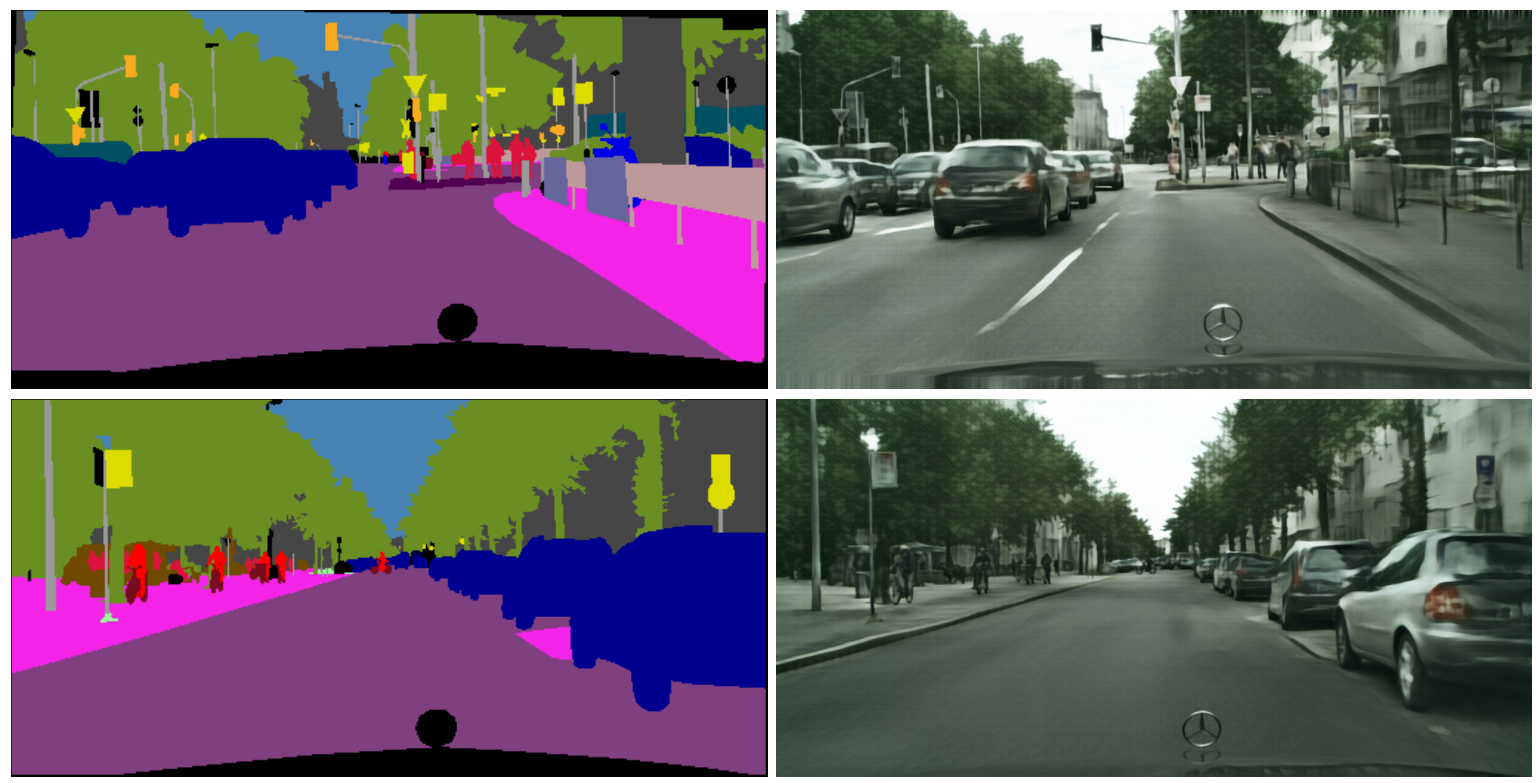
\includegraphics[width=1.0\textwidth]{1.png}
	\end{figure}	
\end{frame}




\begin{frame}{Algorithms}
	\begin{block}{ Architecture}
	 The Cascaded Refinement Network(CRN)
		\begin{figure}
			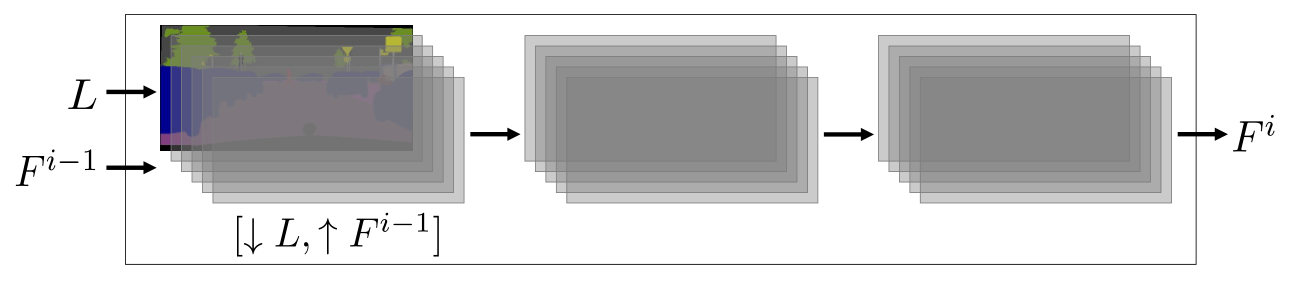
\includegraphics[width=1.0\textwidth]{2.png}
		\end{figure}
	\end{block}
\end{frame}


\begin{frame}{Algorithms}
	\begin{block}{For a training pair $( I , L ) \in \mathcal { D }$, our loss
is}
		\begin{equation}
			\begin{split}
				\mathcal { L } _ { I , L } ( \theta ) = \sum _ { l } \lambda _ { l } \left\| \Phi _ { l } ( I ) - \Phi _ { l } ( g ( L ; \theta ) ) \right\| _ { 1 }
			\end{split}
		\end{equation}
	\end{block}
\end{frame}

\begin{frame}{Algorithms}
	\begin{block}{Our first version of the
modified loss is based on the hindsight loss developed for
multiple choice learning}
		\begin{equation}
			\begin{split}
				\min _ { u } \sum _ { l } \lambda _ { l } \left\| \Phi _ { l } ( I ) - \Phi _ { l } \left( g _ { u } ( L ; \theta ) \right) \right\| _ { 1 }
			\end{split}
		\end{equation}
	\end{block}
	\begin{block}{We now define a more powerful diversity loss as}
		\begin{equation}
			\begin{split}
				\sum _ { p = 1 } ^ { c } \min _ { u } \sum _ { l } \lambda _ { l } \sum _ { j } \left\| L _ { p } ^ { l } \odot \left( \Phi _ { l } ^ { j } ( I ) - \Phi _ { l } ^ { j } \left( g _ { u } ( L ; \theta ) \right) \right) \right\| _ { 1 }
			\end{split}
		\end{equation}
	\end{block}
\end{frame}

\begin{frame}{Experiments}
	\begin{block}{Qualitative comparison on the Cityscapes dataset}
		\begin{figure}
			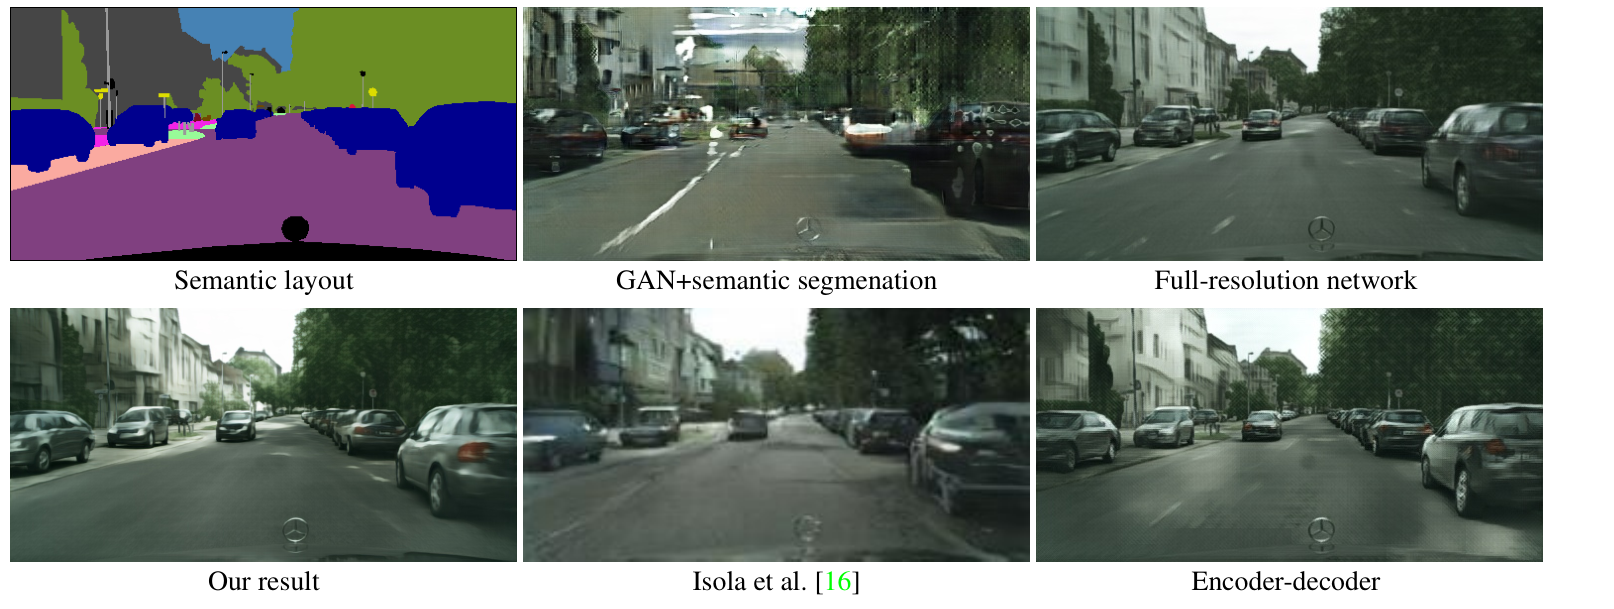
\includegraphics[width=1.0\textwidth]{3.png}
		\end{figure}
	\end{block}
\end{frame}

\begin{frame}{Experiments}
	\begin{block}{Qualitative comparison on the NYU dataset}
		\begin{figure}
			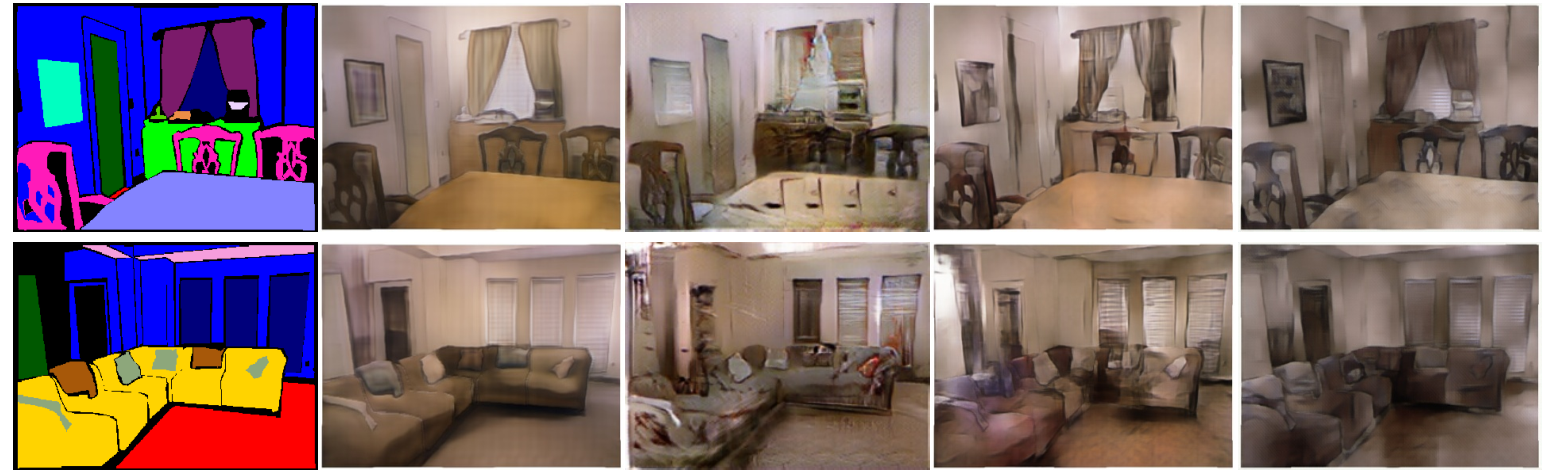
\includegraphics[width=1.0\textwidth]{4.png}
		\end{figure}
	\end{block}
\end{frame}

\begin{frame}{Further}
	\begin{block}{Ongoing Optimization}
		\begin{itemize}
			\item Encoder-decoder and convolutional network have good performance on image processing.
			\item This result, while significantly more realistic than the prior state of the art, are clearly not indistinguishabld from real HD images.
		\end{itemize}
	\end{block}
\end{frame}


\begin{frame}{References}
	\begin{itemize}
		\item Qifeng Chen, Vladlen Koltun. \textit{Photographic Image Synthesis with Cascaded Refinement Networks}
	
	\end{itemize}
\end{frame}




\end{document}
